\q{7}{K-Nearest Bobas} \\ 

Tawainese Pearl Milk Tea (also known as boba) is a very common drink on the Berkeley campus. The two main concentrations of boba cafes are on Southside and Downtown Berkeley. Your friend is a Berkeley boba expert. He says that two useful features for classifying boba are the amount of sugar
(x-axis) and the amount of money (y-axis) for a standard black milk tea with pearls. He identifies several boba places for you, but leaves one unknown boba cafe for you to classify, because he hasn't tried it yet. No two boba places have exactly the same features.

You decide to construct a classifier for the unknown boba cafe using all of the known boba cafes as the training set. Note that the x and y axes have different scales.

\begin{center}
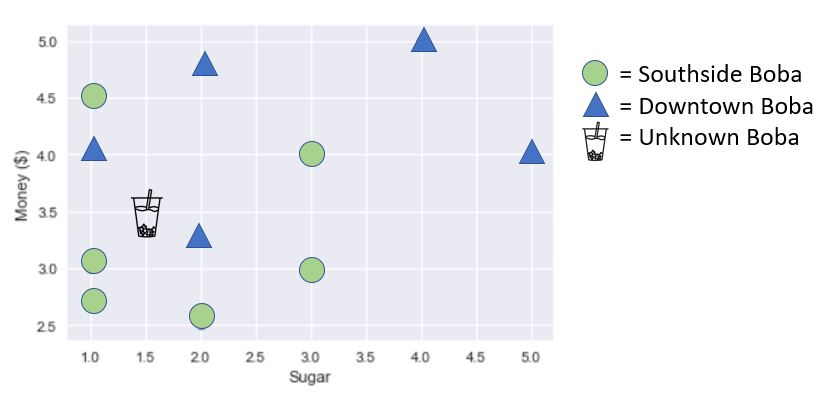
\includegraphics[scale=0.8]{classifiers.JPG}
\end{center}

\begin{enumerate}

\subq{2} Using a 5-nearest neighbor classifier, what would the unknown boba cafe be classified as?
\begin{itemize}[label=\bubble]
\item Southside
\item Downtown
\item Cannot determine
\end{itemize} 

\solution{
	Southside -- 3 southside, 2 downtown
}

\subq{3} What is the problem with using a 4-nearest neighbor classifier for our unknown boba cafe? Provide one possible solution to this problem. \\ \\ \\
\vfill 

\solution{
	It would tie with 2 southside, 2 downtown and then we would need to have a tie breaking scheme
	Any valid tie breaking scheme is accepted -- one could be to choose the class of the point closest, or look at k+1 nearest neighbors when we tie.
}


\subq{2} Every possible pair of feature values for a new boba cafe would be classified as Southside for a 11-nearest neighbor classifier using this training set.
\begin{itemize}[label=\bubble]
\item True
\item False
\item Cannot determine
\end{itemize} 

\solution{
	True. The majority vote will always be southside.
}

\vfill
\end{enumerate}

